% Converted from: Inversion theory.pdf
\documentclass[11pt,a4paper]{article}
\usepackage{notes}
\usepackage{graphicx}
\usetikzlibrary{arrows.meta,calc,decorations.markings,positioning}

\title{Inversion Theory}
\author{Derrick Hasterok}
\date{\today}

\begin{document}
\maketitle

\section{Forward and Inverse Problems}
In geophysical systems there is a \emph{source} and a resulting \emph{field}. Examples:
\begin{itemize}
  \item mass $\rightarrow$ gravity acceleration,
  \item heat production $\rightarrow$ heat flow.
\end{itemize}
The forward problem is written generically as
\begin{equation}
  d = A m ,
\end{equation}
where $m$ is the model (sources), $A$ is the physics operator, and $d$ is the predicted field.

\section{Inverse Problem}
The inverse problem seeks to infer $m$ given measured data $d$. In reality the inverse may not be unique or stable.

\section{Ill-posedness}
Three challenges:
\begin{itemize}
  \item Non-uniqueness -- many models can fit the same data.
  \item Underdetermined systems -- more unknowns than measurements.
  \item Instability -- small data variations produce large model changes.
\end{itemize}

\section{Least Squares Inversion}
Given a linear model $d = A m$, the least-squares estimate solves
\begin{equation}
  (A^T A) m = A^T d .
\end{equation}
The pseudoinverse solution is
\begin{equation}
  m = (A^T A)^{-1} A^T d .
\end{equation}
Weighted least squares uses a diagonal weight matrix $W$ to incorporate uncertainties.

\section{Linear Least Squares in Scalar (Non-Matrix) Form}
\label{sec:scalar-lls}

We begin with the canonical problem of fitting a straight line
\begin{equation}
  y_i \approx m_1 x_i + m_0, \quad i=1,\dots,m,
\end{equation}
by minimizing the sum of squared residuals (misfit)
\begin{equation}
  S(m_0,m_1) = \sum_{i=1}^m \big(y_i - (m_1 x_i + m_0)\big)^2.
\end{equation}
The normal equations follow by setting the partial derivatives to zero:
\begin{align}
  \frac{\partial S}{\partial m_0} &= -2\sum_{i=1}^m \big(y_i - m_1 x_i - m_0\big) = 0, \\
  \frac{\partial S}{\partial m_1} &= -2\sum_{i=1}^m x_i\,\big(y_i - m_1 x_i - m_0\big) = 0.
\end{align}
Rearranging gives the $2\times2$ linear system
\begin{align}
  m\,m_0 + \Big(\sum x_i\Big) m_1 &= \sum y_i, \\
  \Big(\sum x_i\Big) m_0 + \Big(\sum x_i^2\Big) m_1 &= \sum x_i y_i.
\end{align}
Let $\displaystyle S_x=\sum x_i$, $\displaystyle S_y=\sum y_i$, $\displaystyle S_{xx}=\sum x_i^2$, $\displaystyle S_{xy}=\sum x_i y_i$. Then
\begin{align}
  m_1 &= \frac{m S_{xy} - S_x S_y}{m S_{xx} - S_x^2}, \\
  m_0 &= \frac{S_y - m_1 S_x}{m}.
\end{align}
\paragraph{Misfit and residual variance.} With the estimates $\widehat{m}_0,\widehat{m}_1$, residuals are $r_i = y_i - (\widehat{m}_1 x_i + \widehat{m}_0)$ and
\begin{equation}
  S(\widehat{m}_0,\widehat{m}_1) = \sum r_i^2, \qquad
  \widehat{\sigma}^2 = \frac{1}{m-2}\sum r_i^2.
\end{equation}
The parameter covariance (under i.i.d. Gaussian errors) follows from the inverse of the $2\times2$ normal matrix and scales with $\widehat{\sigma}^2$.

\subsection{Weighted Linear Least Squares in Scalar Form}
Suppose each observation has standard deviation $\sigma_i$ (mutually uncorrelated). Define weights $w_i = \sigma_i^{-2}$. Minimize the \emph{weighted} misfit
\begin{equation}
  S_w(m_0,m_1) = \sum_{i=1}^m w_i\,\big(y_i - (m_1 x_i + m_0)\big)^2.
\end{equation}
Set partial derivatives to zero:
\begin{align}
  \frac{\partial S_w}{\partial m_0} &= -2\sum w_i\,\big(y_i - m_1 x_i - m_0\big)=0, \\
  \frac{\partial S_w}{\partial m_1} &= -2\sum w_i x_i\,\big(y_i - m_1 x_i - m_0\big)=0.
\end{align}
Let the weighted sums be $W=\sum w_i$, $S_x^w=\sum w_i x_i$, $S_y^w=\sum w_i y_i$, $S_{xx}^w=\sum w_i x_i^2$, $S_{xy}^w=\sum w_i x_i y_i$. The weighted normal equations are
\begin{align}
  W\,m_0 + S_x^w\,m_1 &= S_y^w, \\
  S_x^w\,m_0 + S_{xx}^w\,m_1 &= S_{xy}^w.
\end{align}
Solving gives
\begin{align}
  m_1 &= \frac{W S_{xy}^w - S_x^w S_y^w}{W S_{xx}^w - (S_x^w)^2}, \\
  m_0 &= \frac{S_y^w - m_1 S_x^w}{W}.
\end{align}
\paragraph{Weighted misfit and uncertainty.} The weighted residuals $r_i=y_i-(\widehat{m}_1 x_i+\widehat{m}_0)$ satisfy
\begin{equation}
  S_w(\widehat{m}_0,\widehat{m}_1) = \sum w_i r_i^2,\qquad
  \widehat{\sigma}^2 = \frac{1}{m-2}\sum w_i r_i^2 \;\Big/\;\Big(\frac{1}{m}\sum w_i\Big),
\end{equation}
where the scaling on $\widehat{\sigma}^2$ reflects an effective variance per datum (alternate unbiased estimators can be used depending on convention). Parameter covariance comes from the inverse of the weighted normal matrix times an appropriate noise scale.

\subsection{Bridge to Matrix Form}
Stack the observations in vectors and matrices:
\begin{equation}
  \mathbf{b}=\begin{bmatrix}y_1\\ \vdots \\ y_m\end{bmatrix},\quad
  \mathbf{A}=\begin{bmatrix}1 & x_1\\ \vdots & \vdots \\ 1 & x_m\end{bmatrix},\quad
  \mathbf{x}=\begin{bmatrix}m_0\\ m_1\end{bmatrix},\quad \mathbf{r}=\mathbf{b}-\mathbf{A}\mathbf{x}.
\end{equation}
Then LLS is $\min\,\|\mathbf{r}\|_2^2$ with normal equations $\mathbf{A}^T\mathbf{A}\,\mathbf{x}=\mathbf{A}^T\mathbf{b}$, and solution $\widehat{\mathbf{x}}=\mathbf{A}^+\mathbf{b}$ (minimum norm when rank-deficient). For the weighted case with uncorrelated errors, let $\mathbf{W}=\mathrm{diag}(w_1^{1/2},\dots,w_m^{1/2})$; then solve
\begin{equation}
  \min\,\|\mathbf{W}(\mathbf{b}-\mathbf{A}\mathbf{x})\|_2^2\quad\Rightarrow\quad
  (\mathbf{A}^T\mathbf{C}_d^{-1}\mathbf{A})\,\mathbf{x}=\mathbf{A}^T\mathbf{C}_d^{-1}\mathbf{b},\quad \mathbf{C}_d^{-1}=\mathbf{W}^T\mathbf{W}.
\end{equation}
This matches the scalar formulas above when $\mathbf{A}$ has the two columns $[\mathbf{1},\,\mathbf{x}]$ and $\mathbf{C}_d=\mathrm{diag}(\sigma_1^2,\dots,\sigma_m^2)$.

\subsection{Scalar Derivation for a General Linear Model}
For $y_i \approx \sum_{j=1}^n a_{ij} x_j$ define
\begin{equation}
  S(\mathbf{x}) = \sum_{i=1}^m \bigg(y_i - \sum_{j=1}^n a_{ij} x_j\bigg)^2.
\end{equation}
Stationarity with respect to $x_k$ gives
\begin{equation}
  \frac{\partial S}{\partial x_k} = -2\sum_{i=1}^m a_{ik}\bigg(y_i - \sum_{j=1}^n a_{ij} x_j\bigg)=0
  \;\;\Rightarrow\;\; \sum_{j=1}^n\Big(\sum_{i=1}^m a_{ik}a_{ij}\Big) x_j = \sum_{i=1}^m a_{ik}y_i,\quad k=1,\dots,n,
\end{equation}
which is precisely $\mathbf{A}^T\mathbf{A}\,\mathbf{x}=\mathbf{A}^T\mathbf{b}$ in component form. The weighted case replaces each summand by $w_i(\cdot)$ and yields $\mathbf{A}^T\mathbf{C}_d^{-1}\mathbf{A}\,\mathbf{x}=\mathbf{A}^T\mathbf{C}_d^{-1}\mathbf{b}$.

\subsection{Notes on Implementation and Pedagogy}
\begin{itemize}
  \item Keep these scalar formulas adjacent to the matrix derivation so students can see the one-to-one mapping.
  \item Use running sums $(S_x,S_{xx},S_{xy},\dots)$ in code examples to mirror the hand derivation.
  \item Present the weighted line fit both ways: (i) as weighted sums, and (ii) as whitening with $\mathbf{W}=\operatorname{diag}(\sigma_i^{-1})$.
  \item When introducing geophysical examples, identify $x_i$ (independent variable), $y_i$ (datum), and link to your forward operator $\mathbf{A}$.
\end{itemize}


% =========================================================
% Linear Least Squares (LLS) and Weighted Least Squares (WLS)
% =========================================================

\section{Linear Least Squares (LLS) and Weighted Least Squares (WLS)}\label{sec:lls-wls}

We collect here the missing foundations for LLS and WLS with explicit intermediate steps, numerical solvers (QR/SVD/Cholesky), geometry, statistics (hat matrix, leverage, uncertainty), and generalized pseudoinverses.

\subsection{Problem Statements}
\paragraph{LLS.} Given $\mathbf{A}\in\mathbb{R}^{m\times n}$, $\mathbf{b}\in\mathbb{R}^m$, find
\[
\min_{\mathbf{x}\in\mathbb{R}^n} \; \|\mathbf{b}-\mathbf{A}\mathbf{x}\|_2^2.
\]
\paragraph{WLS / GLS.} With symmetric positive definite data covariance $\mathbf{C}_d\in\mathbb{R}^{m\times m}$, equivalently weight matrix $\mathbf{W}$ s.t. $\mathbf{W}^T\mathbf{W}=\mathbf{C}_d^{-1}$,
\[
\min_{\mathbf{x}} \; \|\mathbf{b}-\mathbf{A}\mathbf{x}\|_{\mathbf{C}_d^{-1}}^2
= (\mathbf{b}-\mathbf{A}\mathbf{x})^T\mathbf{C}_d^{-1}(\mathbf{b}-\mathbf{A}\mathbf{x})
= \|\tilde{\mathbf{b}}-\tilde{\mathbf{A}}\mathbf{x}\|_2^2,
\]
where $\tilde{\mathbf{A}}=\mathbf{W}\mathbf{A}$ and $\tilde{\mathbf{b}}=\mathbf{W}\mathbf{b}$ (
\emph{whitening}).

\subsection{First-Order Conditions and Normal Equations}
Define $\phi(\mathbf{x})=\tfrac12\|\mathbf{b}-\mathbf{A}\mathbf{x}\|_2^2$. Then
\[
\nabla\phi(\mathbf{x}) = -\mathbf{A}^T(\mathbf{b}-\mathbf{A}\mathbf{x}) = \mathbf{A}^T\mathbf{A}\,\mathbf{x}-\mathbf{A}^T\mathbf{b},\qquad
\nabla^2\phi(\mathbf{x})=\mathbf{A}^T\mathbf{A} \succeq 0.
\]
Setting the gradient to zero yields the normal equations
\[
\boxed{\;\mathbf{A}^T\mathbf{A}\,\mathbf{x}=\mathbf{A}^T\mathbf{b}\;}
\]
For WLS, with $\tilde{\mathbf{A}},\tilde{\mathbf{b}}$ as above,
\[
\boxed{\;\mathbf{A}^T\mathbf{C}_d^{-1}\mathbf{A}\,\mathbf{x}=\mathbf{A}^T\mathbf{C}_d^{-1}\mathbf{b}\;}\,\,\iff\,\,\tilde{\mathbf{A}}^T\tilde{\mathbf{A}}\,\mathbf{x}=\tilde{\mathbf{A}}^T\tilde{\mathbf{b}}.
\]

\subsection{Geometric Interpretation}
Let $\widehat{\mathbf{b}}=\mathbf{A}\widehat{\mathbf{x}}$ be the model fit and $\mathbf{r}=\mathbf{b}-\widehat{\mathbf{b}}$ the residual. The optimality condition is
\[
\mathbf{A}^T\mathbf{r}=\mathbf{0}\quad\iff\quad\mathbf{r}\perp\mathcal{R}(\mathbf{A}).
\]
Thus $\widehat{\mathbf{b}}$ is the \emph{orthogonal projection} of $\mathbf{b}$ onto $\mathcal{R}(\mathbf{A})$. The projector (hat matrix) is
\[
\mathbf{P}=\mathbf{A}\mathbf{A}^+,\qquad \widehat{\mathbf{b}}=\mathbf{P}\mathbf{b},\qquad \mathbf{r}=(\mathbf{I}-\mathbf{P})\,\mathbf{b}.
\]
In WLS with inner product $\langle \mathbf{u},\mathbf{v}\rangle_{\mathbf{C}_d^{-1}}=\mathbf{u}^T\mathbf{C}_d^{-1}\mathbf{v}$ the projector is
\[
\boxed{\;\mathbf{P}_{\mathbf{C}_d^{-1}}=\mathbf{A}(\mathbf{A}^T\mathbf{C}_d^{-1}\mathbf{A})^+\mathbf{A}^T\mathbf{C}_d^{-1}\;}
\]
which is idempotent and self-adjoint in the weighted inner product.

\subsection{Direct Solvers and Numerical Stability}
\paragraph{Avoid forming $\mathbf{A}^T\mathbf{A}$.} It squares the condition number $\kappa(\mathbf{A}^T\mathbf{A})=\kappa(\mathbf{A})^2$; prefer QR or SVD.

\paragraph{QR factorization (LLS).} With thin QR, $\mathbf{A}=\mathbf{Q}\mathbf{R}$ ($\mathbf{Q}\in\mathbb{R}^{m\times n}$ with orthonormal columns, $\mathbf{R}\in\mathbb{R}^{n\times n}$ upper triangular). Then
\[
\min\|\mathbf{b}-\mathbf{Q}\mathbf{R}\mathbf{x}\|_2^2\,\Rightarrow\,\min\|\mathbf{Q}^T\mathbf{b}-\mathbf{R}\mathbf{x}\|_2^2\,\Rightarrow\,\boxed{\;\mathbf{R}\widehat{\mathbf{x}}=\mathbf{Q}^T\mathbf{b}\;}. 
\]
Use Householder or Givens; with column pivoting (QRCP) to reveal rank.

\paragraph{SVD (LLS and rank-deficiency).} $\mathbf{A}=\mathbf{U}\bm{\Sigma}\mathbf{V}^T$ (thin SVD, rank $r$). Minimum-norm solution:
\[
\widehat{\mathbf{x}}=\mathbf{A}^+\mathbf{b}=\sum_{i=1}^r\frac{\mathbf{u}_i^T\mathbf{b}}{\sigma_i}\,\mathbf{v}_i,\qquad \mathbf{A}^+=\mathbf{V}\bm{\Sigma}^{-1}\mathbf{U}^T.
\]
\paragraph{Cholesky (WLS).} For well-conditioned SPD normal matrix $\mathbf{N}=\mathbf{A}^T\mathbf{C}_d^{-1}\mathbf{A}$, factor $\mathbf{N}=\mathbf{L}\mathbf{L}^T$ then solve $\mathbf{L}\mathbf{L}^T\widehat{\mathbf{x}}=\mathbf{A}^T\mathbf{C}_d^{-1}\mathbf{b}$. Alternatively, whiten first and use QR/SVD on $\tilde{\mathbf{A}}$.

\subsection{Statistical View: Hat Matrix, Leverage, Covariances}
Assume $\mathbf{b}=\mathbf{A}\mathbf{x}_\star+\boldsymbol{\varepsilon}$ with $\mathbb{E}[\boldsymbol{\varepsilon}]=\mathbf{0}$, $\operatorname{Cov}(\boldsymbol{\varepsilon})=\sigma^2\mathbf{I}$ (LLS) or $\mathbf{C}_d$ (WLS).
\paragraph{Hat matrix.} In LLS, $\mathbf{H}=\mathbf{P}=\mathbf{A}\mathbf{A}^+$. Diagonal entries $h_{ii}$ are \emph{leverages} (influence). Residuals satisfy $\mathbb{E}[\mathbf{r}]=\mathbf{0}$ and $\operatorname{Cov}(\mathbf{r})=(\mathbf{I}-\mathbf{H})\,\sigma^2$.
\paragraph{BLUE / GLS.} The WLS estimator
\[
\widehat{\mathbf{x}}=(\mathbf{A}^T\mathbf{C}_d^{-1}\mathbf{A})^{-1}\mathbf{A}^T\mathbf{C}_d^{-1}\mathbf{b}
\]
(if full column rank) is the \emph{best linear unbiased estimator} (BLUE). Its covariance is
\[
\operatorname{Cov}(\widehat{\mathbf{x}})=(\mathbf{A}^T\mathbf{C}_d^{-1}\mathbf{A})^{-1}.
\]
For unknown scale, an unbiased $\hat{\sigma}^2=\|\mathbf{W}(\mathbf{b}-\mathbf{A}\widehat{\mathbf{x}})\|_2^2/(m-n)$ yields $\widehat{\operatorname{Cov}}(\widehat{\mathbf{x}})=\hat{\sigma}^2(\mathbf{A}^T\mathbf{C}_d^{-1}\mathbf{A})^{-1}$.

\subsection{Generalized Pseudoinverse under Metrics}
Define data inner product $\langle \cdot,\cdot\rangle_{\mathbf{C}_d^{-1}}$ and model inner product $\langle \cdot,\cdot\rangle_{\mathbf{C}_m^{-1}}$ with SPD $\mathbf{C}_d,\mathbf{C}_m$.
Among all minimizers of WLS, the one of minimal $\|\mathbf{x}\|_{\mathbf{C}_m^{-1}}$ is
\[
\boxed{\;\widehat{\mathbf{x}}=\mathbf{C}_m\mathbf{A}^T\mathbf{C}_d^{-1}\,\big(\mathbf{A}\mathbf{C}_m\mathbf{A}^T\big)^{+}\,\mathbf{b}\;}\,.
\]
Under whitening with $\mathbf{W}^T\mathbf{W}=\mathbf{C}_d^{-1}$, this is $\widehat{\mathbf{x}}=\mathbf{C}_m\tilde{\mathbf{A}}^T(\tilde{\mathbf{A}}\mathbf{C}_m\tilde{\mathbf{A}}^T)^+\tilde{\mathbf{b}}$.

\subsection{Rank-Deficient and Constrained Problems}
\paragraph{Rank-deficient LLS/WLS.} When $\operatorname{rank}(\mathbf{A})=r<n$, the minimum-norm solution is provided by the (weighted) pseudoinverse formulas above; TSVD or Tikhonov can regularize:
\[
\min_{\mathbf{x}}\; \|\tilde{\mathbf{b}}-\tilde{\mathbf{A}}\mathbf{x}\|_2^2 + \lambda^2\|\mathbf{L}\mathbf{x}\|_2^2.
\]
\paragraph{Equality-constrained LLS.} For $\mathbf{C}\mathbf{x}=\mathbf{d}$, form KKT system
\[
\begin{bmatrix}
\mathbf{A}^T\mathbf{A} & \mathbf{C}^T\\
\mathbf{C} & \mathbf{0}
\end{bmatrix}
\begin{bmatrix}
\mathbf{x}\\ \boldsymbol{\lambda}
\end{bmatrix}
=
\begin{bmatrix}
\mathbf{A}^T\mathbf{b}\\ \mathbf{d}
\end{bmatrix},
\]
or eliminate in a null-space basis for numerical stability.

\subsection{TikZ: Weighted Projection Geometry}
\begin{figure}[h!]
\centering
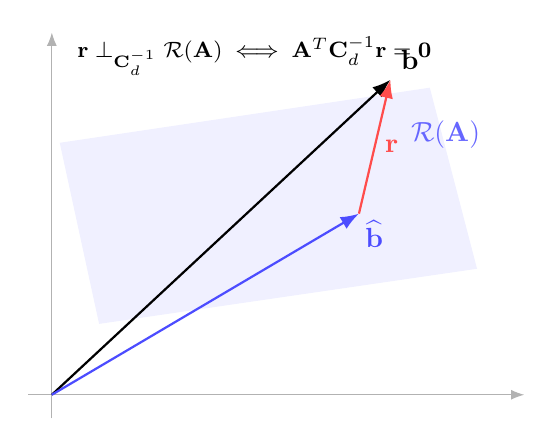
\begin{tikzpicture}[scale=1.0,>=Latex]
  % Data axes
  \draw[->,gray!60] (-0.3,0) -- (6.0,0);
  \draw[->,gray!60] (0,-0.3) -- (0,4.6);

  % Subspace R(A)
  \fill[blue!6] (0.6,0.9) -- (5.4,1.6) -- (4.8,3.9) -- (0.1,3.2) -- cycle;
  \node[blue!60] at (5.0,3.3) {$\mathcal{R}(\mathbf{A})$};

  % b and projection in weighted sense
  \coordinate (O) at (0,0);
  \coordinate (b) at (4.3,4.0);
  \draw[->,thick] (O) -- (b) node[above right] {$\mathbf{b}$};

  % Weighted projection point (visual)
  \coordinate (bh) at (3.9,2.3);
  \draw[->,thick,blue!70] (O) -- (bh) node[below right=-2pt] {$\widehat{\mathbf{b}}$};
  \draw[->,thick,red!70] (bh) -- (b) node[midway,right] {$\mathbf{r}$};

  % A note on metric
  \node[align=left,anchor=west] at (0.2,4.3) {\footnotesize $\mathbf{r}\perp_{\mathbf{C}_d^{-1}}\mathcal{R}(\mathbf{A})\iff \mathbf{A}^T\mathbf{C}_d^{-1}\mathbf{r}=\mathbf{0}$};
\end{tikzpicture}
\caption{Weighted orthogonal projection of $\mathbf{b}$ onto $\mathcal{R}(\mathbf{A})$ under the $\mathbf{C}_d^{-1}$ inner product.}
\end{figure}

\subsection{Computation and Conditioning Details}
\begin{itemize}
  \item \textbf{Scaling and preconditioning}: Scale columns of $\mathbf{A}$ and variables to balance magnitudes; left-precondition with $\mathbf{W}$ (whitening) in WLS.
  \item \textbf{QR with column pivoting (QRCP)}: Detects numerical rank; solves least squares in the leading subspace.
  \item \textbf{SVD filter factors}: For ridge/Tikhonov with parameter $\lambda$, the solution is $\sum_i \phi_i(\lambda)(\mathbf{u}_i^T\tilde{\mathbf{b}})\mathbf{v}_i$ with $\phi_i=\sigma_i/(\sigma_i^2+\lambda^2)$.
  \item \textbf{Uncertainty quantification}: Report standard deviations from diagonal of $(\mathbf{A}^T\mathbf{C}_d^{-1}\mathbf{A})^{-1}$, scaled by $\hat{\sigma}^2$.
  \item \textbf{Outliers / robust LS}: Replace $\ell_2$ with M-estimators; solved by iteratively reweighted least squares (IRLS).
\end{itemize}

\subsection*{References}
% Classic, stable references for LS/WLS and numerics
\begin{itemize}
  \item G. H. Golub and C. F. Van Loan, \emph{Matrix Computations}, 4th ed., JHU Press, 2013.
  \item \AA. Bj\"orck, \emph{Numerical Methods for Least Squares Problems}, SIAM, 1996.
  \item R. A. Horn and C. R. Johnson, \emph{Matrix Analysis}, 2nd ed., Cambridge Univ. Press, 2012.
  \item S. M. Kay, \emph{Fundamentals of Statistical Signal Processing, Vol. I}, Prentice Hall, 1993 (BLUE/GLS viewpoint).
\end{itemize}


% =========================================================
% Jacobian Geometry, Pseudoinverse, and Regularization
% =========================================================

\section{Jacobian Geometry, Pseudoinverse, and Regularization}

\subsection{From Nonlinear to Linearized Least Squares}
Consider a nonlinear forward model $\mathbf{f}(\mathbf{m}) \in \mathbb{R}^m$ with data $\mathbf{d}\in\mathbb{R}^m$ and parameters $\mathbf{m}\in\mathbb{R}^n$. The Gauss--Newton linearization at $\mathbf{m}_k$ gives
\[
\mathbf{f}(\mathbf{m}_k+\delta\mathbf{m}) \approx \mathbf{f}(\mathbf{m}_k) + \mathbf{J}_k\,\delta\mathbf{m},
\]
where $\mathbf{J}_k = \left.\frac{\partial \mathbf{f}}{\partial \mathbf{m}}\right|_{\mathbf{m}_k}$ is the Jacobian. The linearized least-squares problem for the update $\delta\mathbf{m}$ is
\[
\min_{\delta\mathbf{m}} \; \|\mathbf{r}_k - \mathbf{J}_k \delta\mathbf{m}\|_2^2,
\qquad \text{with} \quad \mathbf{r}_k = \mathbf{d} - \mathbf{f}(\mathbf{m}_k).
\]
Its normal equations are
\[
\mathbf{J}_k^\top \mathbf{J}_k \,\delta\mathbf{m} = \mathbf{J}_k^\top \mathbf{r}_k.
\]
Under full column rank, the unique least-squares update is
\[
\delta\mathbf{m} = \mathbf{J}_k^{+}\,\mathbf{r}_k,
\]
where $\mathbf{J}_k^{+}$ is the Moore--Penrose pseudoinverse (see \S\ref{subsec:pseudo}).

\subsection{Geometric View: Column Space, Projection, and Orthogonality}
Let $\mathcal{R}(\mathbf{J})$ denote the column space of $\mathbf{J}\in\mathbb{R}^{m\times n}$ (with $m\ge n$ typically). The least-squares solution determines the projection of the data $\mathbf{y}=\mathbf{r}_k$ onto $\mathcal{R}(\mathbf{J})$:
\[
\widehat{\mathbf{y}} = \mathbf{J}\,\delta\mathbf{m} \in \mathcal{R}(\mathbf{J}), \qquad
\mathbf{r} = \mathbf{y} - \widehat{\mathbf{y}} \in \mathcal{R}(\mathbf{J})^\perp.
\]
Equivalently,
\[
\mathbf{J}^\top \mathbf{r} = \mathbf{0}, \quad \text{i.e., the residual is orthogonal to every column of } \mathbf{J}.
\]

\subsubsection*{TikZ: Geometry of Least Squares in Data Space}
\begin{figure}[h!]
\centering
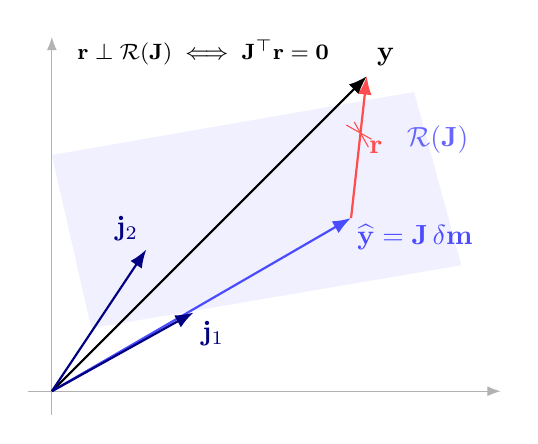
\begin{tikzpicture}[scale=1.0,>=Latex]
  % Axes (for visual reference)
  \draw[->,gray!60] (-0.3,0) -- (5.7,0) node[below] {};
  \draw[->,gray!60] (0,-0.3) -- (0,4.5) node[left] {};

  % A 2D subspace (a slanted plane segment in R^m)
  \fill[blue!6] (0.5,0.8) -- (5.2,1.6) -- (4.6,3.8) -- (0,3.0) -- cycle;
  \node[blue!60] at (4.9,3.2) {$\mathcal{R}(\mathbf{J})$};

  % Data vector y
  \coordinate (O) at (0,0);
  \coordinate (Y) at (4.0,4.0);
  \draw[->,thick] (O) -- (Y) node[above right] {$\mathbf{y}$};

  % Projection y_hat onto subspace
  % Choose a point roughly inside the blue polygon
  \coordinate (Yhat) at (3.8,2.2);
  \draw[->,thick,blue!70] (O) -- (Yhat) node[below right=-2pt] {$\widehat{\mathbf{y}}=\mathbf{J}\,\delta\mathbf{m}$};

  % Residual r = y - yhat (orthogonal to subspace)
  \draw[->,thick,red!70] (Yhat) -- (Y) node[midway,right] {$\mathbf{r}$};

  % Orthogonality marker
  \draw[red!70] ($(Yhat)!0.6!(Y)$) ++(-0.18,0.10) -- ++(0.32,-0.18);
  \draw[red!70] ($(Yhat)!0.6!(Y)$) ++(0.10,-0.18) -- ++(-0.18,0.32);

  % A couple of columns of J as directions in the subspace
  \coordinate (c1) at (1.8,1.0);
  \coordinate (c2) at (1.2,1.8);
  \draw[->,blue!50!black,thick] (O) -- (c1) node[below right=-1pt] {$\mathbf{j}_1$};
  \draw[->,blue!50!black,thick] (O) -- (c2) node[above left=-1pt] {$\mathbf{j}_2$};

  % Caption-esque labels
  \node[align=left,anchor=west] at (0.2,4.3) {\footnotesize $\mathbf{r}\perp \mathcal{R}(\mathbf{J}) \iff \mathbf{J}^\top \mathbf{r}=\mathbf{0}$};
\end{tikzpicture}
\caption{Least-squares geometry: $\widehat{\mathbf{y}}$ is the orthogonal projection of $\mathbf{y}$ onto $\mathcal{R}(\mathbf{J})$, with residual $\mathbf{r}$ orthogonal to the column space of $\mathbf{J}$.}
\end{figure}

\subsection{Normal Equations and Conditioning}
Expanding the objective,
\[
\|\mathbf{y}-\mathbf{J}\,\delta\mathbf{m}\|_2^2
= \mathbf{y}^\top\mathbf{y} - 2\,\delta\mathbf{m}^\top \mathbf{J}^\top \mathbf{y}
+ \delta\mathbf{m}^\top (\mathbf{J}^\top \mathbf{J}) \delta\mathbf{m}.
\]
Setting the gradient to zero yields $\mathbf{J}^\top \mathbf{J}\,\delta\mathbf{m}=\mathbf{J}^\top \mathbf{y}$.
If $\mathbf{J}$ is ill-conditioned or rank-deficient, $\mathbf{J}^\top \mathbf{J}$ is more ill-conditioned (squared condition number). This motivates SVD-based solutions and regularization.

\subsection{The Pseudoinverse in Detail}\label{subsec:pseudo}
Let the thin SVD of $\mathbf{J}\in\mathbb{R}^{m\times n}$ (rank $r$) be
\[
\mathbf{J} = \mathbf{U}\,\bm{\Sigma}\,\mathbf{V}^\top, \quad
\mathbf{U}\in\mathbb{R}^{m\times r},\; \mathbf{V}\in\mathbb{R}^{n\times r},\;
\bm{\Sigma}=\mathrm{diag}(\sigma_1,\ldots,\sigma_r),\; \sigma_1\ge\cdots\ge\sigma_r>0.
\]
The Moore--Penrose pseudoinverse is
\[
\mathbf{J}^+ = \mathbf{V}\,\bm{\Sigma}^{-1}\,\mathbf{U}^\top,
\]
and the \emph{minimum-norm} least-squares solution (for underdetermined or rank-deficient cases) is
\[
\delta\mathbf{m}^* = \mathbf{J}^+\,\mathbf{y}
= \sum_{i=1}^r \frac{\mathbf{u}_i^\top \mathbf{y}}{\sigma_i}\,\mathbf{v}_i.
\]
\paragraph{Moore--Penrose conditions.} $\mathbf{J}^+$ is the unique matrix satisfying
\[
\mathbf{J}\mathbf{J}^+\mathbf{J}=\mathbf{J},\quad
\mathbf{J}^+\mathbf{J}\mathbf{J}^+=\mathbf{J}^+,\quad
(\mathbf{J}\mathbf{J}^+)^\top=\mathbf{J}\mathbf{J}^+,\quad
(\mathbf{J}^+\mathbf{J})^\top=\mathbf{J}^+\mathbf{J}.
\]
\paragraph{Geometry.} $\mathbf{J}^+$ maps data to parameters via the right singular vectors, scaling by $1/\sigma_i$, and discarding any component in the left-null space of $\mathbf{J}^\top$. Small singular values amplify noise; regularization damps these directions.

\subsubsection*{TikZ: SVD / Pseudoinverse Mapping Geometry}
\begin{figure}[h!]
\centering
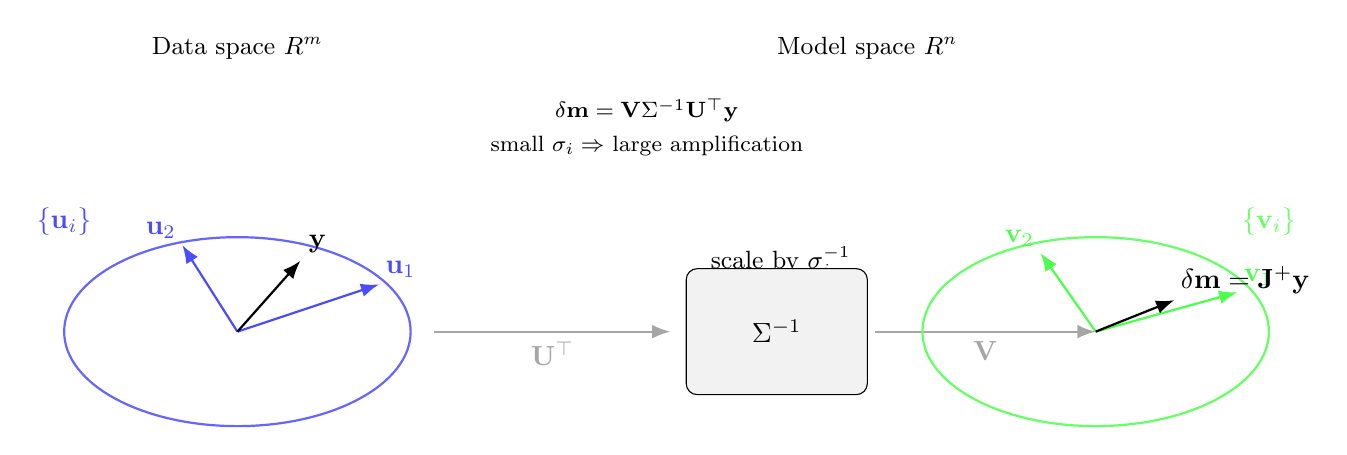
\begin{tikzpicture}[scale=1.0,>=Latex]
  % Two panels: data space (left) and model space (right)
  \node at (0,3.6) {\small Data space $\mathbb{R}^m$};
  \node at (8,3.6) {\small Model space $\mathbb{R}^n$};

  % Ellipse in data space showing left singular vectors
  \draw[thick,blue!60] (0,0) ellipse (2.2cm and 1.2cm);
  \node[blue!70] at (-2.2,1.4) {$\{\mathbf{u}_i\}$};

  % Basis vectors u1, u2 drawn
  \draw[->,thick,blue!70] (0,0) -- (1.8,0.6) node[above right=-2pt] {$\mathbf{u}_1$};
  \draw[->,thick,blue!70] (0,0) -- (-0.7,1.1) node[above left=-2pt] {$\mathbf{u}_2$};

  % Data vector y
  \coordinate (Y) at (0.8,0.9);
  \draw[->,thick] (0,0) -- (Y) node[above right=-1pt] {$\mathbf{y}$};

  % Arrow showing mapping by U^T (coordinates)
  \draw[->,gray!70,thick] (2.5,0.0) -- (5.5,0.0) node[midway,below] {$\mathbf{U}^\top$};

  % Middle panel: singular value scaling
  \node at (6.9,0.9) {\small scale by $\sigma_i^{-1}$};
  \draw[fill=gray!10,rounded corners] (5.7,-0.8) rectangle (8.0,0.8);
  \node at (6.85,0.0) {$\bm{\Sigma}^{-1}$};

  % Arrow to model space
  \draw[->,gray!70,thick] (8.1,0.0) -- (10.9,0.0) node[midway,below] {$\mathbf{V}$};

  % Model space ellipse showing right singular vectors v_i
  \begin{scope}[shift={(8,0)}]
    \draw[thick,green!60] (2.9,0) ellipse (2.2cm and 1.2cm);
    \node[green!60] at (5.1,1.4) {$\{\mathbf{v}_i\}$};
    \draw[->,thick,green!70] (2.9,0) -- (4.7,0.5) node[above right=-2pt] {$\mathbf{v}_1$};
    \draw[->,thick,green!70] (2.9,0) -- (2.2,1.0) node[above left=-2pt] {$\mathbf{v}_2$};
    % Solution vector delta m
    \coordinate (M) at (3.9,0.4);
    \draw[->,thick] (2.9,0) -- (M) node[above right=-2pt] {$\delta\mathbf{m}=\mathbf{J}^+\mathbf{y}$};
  \end{scope}

  % Notes
  \node[align=center] at (5.2,2.6) {\footnotesize $\delta\mathbf{m}=\mathbf{V}\bm{\Sigma}^{-1}\mathbf{U}^\top\mathbf{y}$\\
  \footnotesize small $\sigma_i \Rightarrow$ large amplification};
\end{tikzpicture}
\caption{Pseudoinverse via SVD: project $\mathbf{y}$ onto $\{\mathbf{u}_i\}$, scale by $1/\sigma_i$, then map into model space via $\{\mathbf{v}_i\}$.}
\end{figure}

\subsection{Regularization}\label{subsec:reg}
When $\mathbf{J}$ is ill-conditioned or rank-deficient, we stabilize the inversion by augmenting the objective with prior information or penalties.

\subsubsection{Tikhonov ($\ell_2$) Regularization}
\paragraph{Zero-order (ridge).}
\[
\min_{\delta\mathbf{m}} \; \|\mathbf{y}-\mathbf{J}\delta\mathbf{m}\|_2^2 + \lambda^2 \,\|\delta\mathbf{m}\|_2^2.
\]
Normal equations:
\[
\left(\mathbf{J}^\top \mathbf{J} + \lambda^2 \mathbf{I}\right)\delta\mathbf{m} = \mathbf{J}^\top \mathbf{y}.
\]
SVD filter factors:
\[
\delta\mathbf{m}_\lambda = \sum_{i=1}^r \frac{\sigma_i}{\sigma_i^2+\lambda^2}\,(\mathbf{u}_i^\top \mathbf{y})\,\mathbf{v}_i,
\qquad
\phi_i(\lambda)=\frac{\sigma_i}{\sigma_i^2+\lambda^2}.
\]
Small singular directions are damped smoothly as $\sigma_i \downarrow 0$.

\paragraph{General-order (with roughness operator).}
Let $\mathbf{L}$ encode roughness (e.g., discrete gradient or Laplacian on the model):
\[
\min_{\delta\mathbf{m}} \; \|\mathbf{y}-\mathbf{J}\delta\mathbf{m}\|_2^2 + \lambda^2 \,\|\mathbf{L}\,\delta\mathbf{m}\|_2^2,
\]
with normal equations
\[
\big(\mathbf{J}^\top \mathbf{J} + \lambda^2 \mathbf{L}^\top \mathbf{L}\big)\,\delta\mathbf{m} = \mathbf{J}^\top \mathbf{y}.
\]
This biases solutions toward smoothness or other desired structure.

\subsubsection{Levenberg--Marquardt (Damped Gauss--Newton)}
For nonlinear problems, LM uses
\[
\left(\mathbf{J}^\top\mathbf{J} + \lambda^2 \mathbf{D}\right)\delta\mathbf{m} = \mathbf{J}^\top \mathbf{r},
\]
with $\mathbf{D}$ often chosen as $\mathrm{diag}(\mathbf{J}^\top \mathbf{J})$ (Marquardt) or $\mathbf{I}$ (Levenberg). The damping $\lambda$ is adapted: large $\lambda$ gives gradient-descent-like steps; small $\lambda$ recovers Gauss--Newton near the solution.

\subsubsection{Truncated SVD (TSVD)}
Solve in the dominant subspace spanned by the first $k$ singular vectors:
\[
\delta\mathbf{m}_{\text{TSVD}} = \sum_{i=1}^{k} \frac{\mathbf{u}_i^\top \mathbf{y}}{\sigma_i}\,\mathbf{v}_i.
\]
Acts as a hard spectral cutoff; useful when the spectrum decays rapidly or is noisy beyond rank $k$.

\subsubsection{Sparsity-Promoting ($\ell_1$) Regularization (brief)}
\[
\min_{\delta\mathbf{m}} \; \|\mathbf{y}-\mathbf{J}\delta\mathbf{m}\|_2^2 + \lambda \|\mathbf{W}\delta\mathbf{m}\|_1,
\]
with $\mathbf{W}$ possibly a wavelet or transform promoting sparsity. Solved by proximal/iterative schemes (ISTA/FISTA/ADMM). Often yields sharp, piecewise-constant structure.

\subsection{Choosing \texorpdfstring{$\lambda$}{lambda}}
Common strategies:
\begin{itemize}
  \item \emph{L-curve}: plot $\log \|\mathbf{y}-\mathbf{J}\delta\mathbf{m}_\lambda\|$ vs.\ $\log \|\mathbf{L}\delta\mathbf{m}_\lambda\|$ and pick the corner.
  \item \emph{Generalized Cross-Validation (GCV)}: minimize a predictive risk proxy (especially for $\ell_2$).
  \item \emph{Discrepancy Principle}: choose $\lambda$ so that the residual norm matches the expected noise level.
\end{itemize}

\subsection{Intermediate Derivations (Expanded)}
\paragraph{Gradient and Hessian of the linearized objective.}
\[
\Phi(\delta\mathbf{m}) = \|\mathbf{y}-\mathbf{J}\delta\mathbf{m}\|_2^2
= (\mathbf{y}-\mathbf{J}\delta\mathbf{m})^\top(\mathbf{y}-\mathbf{J}\delta\mathbf{m}).
\]
Then
\[
\nabla \Phi = -2\,\mathbf{J}^\top (\mathbf{y}-\mathbf{J}\delta\mathbf{m}) 
= -2\,\mathbf{J}^\top \mathbf{y} + 2\,\mathbf{J}^\top\mathbf{J}\,\delta\mathbf{m},
\]
\[
\nabla^2 \Phi = 2\,\mathbf{J}^\top \mathbf{J}.
\]
Setting $\nabla\Phi=\mathbf{0}$ recovers the normal equations.

\paragraph{Equivalence of normal equations and projection.}
The optimality condition $\mathbf{J}^\top(\mathbf{y}-\widehat{\mathbf{y}})=\mathbf{0}$ says $\mathbf{y}-\widehat{\mathbf{y}}\perp \mathcal{R}(\mathbf{J})$, thus $\widehat{\mathbf{y}}$ is the orthogonal projection of $\mathbf{y}$ onto $\mathcal{R}(\mathbf{J})$. The projector is $\mathbf{P}_{\mathcal{R}(\mathbf{J})}=\mathbf{J}\mathbf{J}^+$ (symmetric idempotent). Hence
\[
\widehat{\mathbf{y}} = \mathbf{P}_{\mathcal{R}(\mathbf{J})}\,\mathbf{y}=\mathbf{J}\mathbf{J}^+ \mathbf{y},\quad
\mathbf{r} = (\mathbf{I}-\mathbf{J}\mathbf{J}^+)\mathbf{y}.
\]

\paragraph{SVD-based solution avoids squaring the condition number.}
Directly solving $\min\|\mathbf{y}-\mathbf{J}\delta\mathbf{m}\|_2$ via SVD yields better numerical stability than solving $\mathbf{J}^\top \mathbf{J}\,\delta\mathbf{m}=\mathbf{J}^\top \mathbf{y}$, because $\kappa(\mathbf{J}^\top\mathbf{J})=\kappa(\mathbf{J})^2$.

\subsection{TikZ: Normal vs.\ Regularized Normal Equations}
\begin{figure}[h!]
\centering
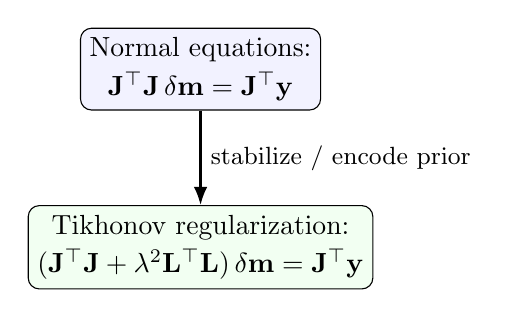
\begin{tikzpicture}[>=Latex]
  \node[draw,rounded corners,fill=blue!5,align=center] (NE)
    {Normal equations:\\[2pt]
     $\mathbf{J}^\top\mathbf{J}\,\delta\mathbf{m}=\mathbf{J}^\top\mathbf{y}$};

  \node[draw,rounded corners,fill=green!5,align=center,below=1.2cm of NE] (REG)
    {Tikhonov regularization:\\[2pt]
     $(\mathbf{J}^\top\mathbf{J}+\lambda^2\mathbf{L}^\top\mathbf{L})\,\delta\mathbf{m}=\mathbf{J}^\top\mathbf{y}$};

  \draw[->,thick] (NE) -- (REG) node[midway,right] {\small stabilize / encode prior};
\end{tikzpicture}
\caption{Regularization augments the normal equations to improve conditioning and encode prior structure.}
\end{figure}

\subsection{Practical Notes}
\begin{itemize}
  \item \textbf{Scaling}: Normalize columns of $\mathbf{J}$ and/or parameters to balance sensitivities.
  \item \textbf{Whitening}: If data covariance is $\mathbf{C}_d$, prewhiten with $\mathbf{C}_d^{-1/2}$ so residuals are in units of standard deviations.
  \item \textbf{Rank-revealing factorizations}: Use SVD or QR with column pivoting to detect rank deficiency and guide TSVD or damping.
  \item \textbf{Stop criteria}: use relative step size $\|\delta\mathbf{m}\|/\|\mathbf{m}\|$, relative residual decrease, and/or gradient norm $\|\mathbf{J}^\top \mathbf{r}\|$.
\end{itemize}

\section{Newton's Method for Nonlinear Problems}
For nonlinear $f(m)$, linearize around model iteration $m_k$ using the Jacobian $J$:
\begin{equation}
  f(m_k) + J_k \Delta m = d .
\end{equation}
Solve for $\Delta m$ and update
\begin{equation}
  m_{k+1} = m_k + \Delta m .
\end{equation}
Iterate until the misfit is below tolerance.

\section{Jacobian Geometry, Pseudoinverse, and Regularization}

\subsection{From Nonlinear to Linearized Least Squares}
Consider a nonlinear forward model $\mathbf{f}(\mathbf{m}) \in \mathbb{R}^m$ with data $\mathbf{d}\in\mathbb{R}^m$ and parameters $\mathbf{m}\in\mathbb{R}^n$. The Gauss--Newton linearization at $\mathbf{m}_k$ gives
\[
\mathbf{f}(\mathbf{m}_k+\delta\mathbf{m}) \approx \mathbf{f}(\mathbf{m}_k) + \mathbf{J}_k\,\delta\mathbf{m},
\]
where $\mathbf{J}_k = \left.\frac{\partial \mathbf{f}}{\partial \mathbf{m}}\right|_{\mathbf{m}_k}$ is the Jacobian. The linearized least-squares problem for the update $\delta\mathbf{m}$ is
\[
\min_{\delta\mathbf{m}} \; \|\mathbf{r}_k - \mathbf{J}_k \, \delta\mathbf{m}\|_2^2, \qquad \text{with} \quad \mathbf{r}_k = \mathbf{d} - \mathbf{f}(\mathbf{m}_k).
\]
Its normal equations are
\[
\mathbf{J}_k^\top \mathbf{J}_k \,\delta\mathbf{m} = \mathbf{J}_k^\top \mathbf{r}_k.
\]
Under full column rank, the unique least-squares update is $\delta\mathbf{m} = \mathbf{J}_k^{+}\,\mathbf{r}_k$ where $\mathbf{J}_k^{+}$ is the Moore--Penrose pseudoinverse (see \S\ref{subsec:pseudo}).

\subsection{Geometric View: Column Space, Projection, and Orthogonality}
Let $\mathcal{R}(\mathbf{J})$ denote the column space of $\mathbf{J}\in\mathbb{R}^{m\times n}$ (with $m\ge n$ typically). The least-squares solution determines the projection of the data $\mathbf{y}=\mathbf{r}_k$ onto $\mathcal{R}(\mathbf{J})$:
\[
\widehat{\mathbf{y}} = \mathbf{J}\,\delta\mathbf{m} \in \mathcal{R}(\mathbf{J}), \qquad
\mathbf{r} = \mathbf{y} - \widehat{\mathbf{y}} \in \mathcal{R}(\mathbf{J})^\perp.
\]
Equivalently, $\mathbf{J}^\top \mathbf{r} = \mathbf{0}$, i.e., the residual is orthogonal to every column of $\mathbf{J}$.

\subsubsection*{TikZ: Geometry of Least Squares in Data Space}
\begin{figure}[h!]
\centering
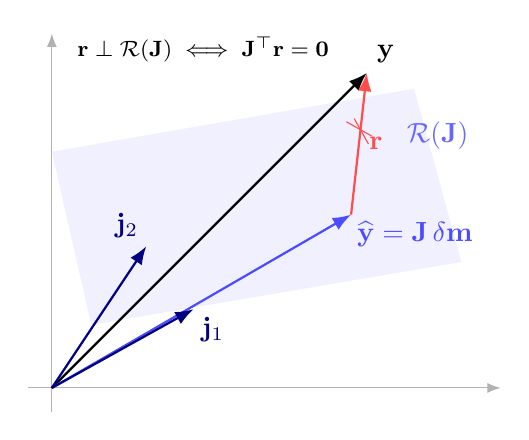
\begin{tikzpicture}[scale=1.0,>=Latex]
  % Axes
  \draw[->,gray!60] (-0.3,0) -- (5.7,0);
  \draw[->,gray!60] (0,-0.3) -- (0,4.5);

  % A 2D subspace (a slanted plane segment in R^m)
  \fill[blue!6] (0.5,0.8) -- (5.2,1.6) -- (4.6,3.8) -- (0,3.0) -- cycle;
  \node[blue!60] at (4.9,3.2) {$\mathcal{R}(\mathbf{J})$};

  % Vectors
  \coordinate (O) at (0,0);
  \coordinate (Y) at (4.0,4.0);
  \draw[->,thick] (O) -- (Y) node[above right] {$\mathbf{y}$};

  \coordinate (Yhat) at (3.8,2.2);
  \draw[->,thick,blue!70] (O) -- (Yhat) node[below right=-2pt] {$\widehat{\mathbf{y}}=\mathbf{J}\,\delta\mathbf{m}$};

  \draw[->,thick,red!70] (Yhat) -- (Y) node[midway,right] {$\mathbf{r}$};

  % Orthogonality marker
  \draw[red!70] ($(Yhat)!0.6!(Y)$) ++(-0.18,0.10) -- ++(0.32,-0.18);
  \draw[red!70] ($(Yhat)!0.6!(Y)$) ++(0.10,-0.18) -- ++(-0.18,0.32);

  % A couple of columns of J as directions
  \coordinate (c1) at (1.8,1.0);
  \coordinate (c2) at (1.2,1.8);
  \draw[->,blue!50!black,thick] (O) -- (c1) node[below right=-1pt] {$\mathbf{j}_1$};
  \draw[->,blue!50!black,thick] (O) -- (c2) node[above left=-1pt] {$\mathbf{j}_2$};

  \node[align=left,anchor=west] at (0.2,4.3) {\footnotesize $\mathbf{r}\perp \mathcal{R}(\mathbf{J}) \iff \mathbf{J}^\top \mathbf{r}=\mathbf{0}$};
\end{tikzpicture}
\caption{Least-squares geometry: $\widehat{\mathbf{y}}$ is the orthogonal projection of $\mathbf{y}$ onto $\mathcal{R}(\mathbf{J})$, with residual $\mathbf{r}$ orthogonal to the column space of $\mathbf{J}$.}
\end{figure}

\subsection{Normal Equations and Conditioning}
Expanding the objective,
\[
\|\mathbf{y}-\mathbf{J}\,\delta\mathbf{m}\|_2^2
= \mathbf{y}^\top\mathbf{y} - 2\,\delta\mathbf{m}^\top \mathbf{J}^\top \mathbf{y}
+ \delta\mathbf{m}^\top (\mathbf{J}^\top \mathbf{J}) \delta\mathbf{m}.
\]
Setting the gradient to zero yields $\mathbf{J}^\top \mathbf{J}\,\delta\mathbf{m}=\mathbf{J}^\top \mathbf{y}$. If $\mathbf{J}$ is ill-conditioned or rank-deficient, $\mathbf{J}^\top \mathbf{J}$ is more ill-conditioned (squared condition number). This motivates SVD-based solutions and regularization.

\subsection{The Pseudoinverse in Detail}\label{subsec:pseudo}
Let the thin SVD of $\mathbf{J}\in\mathbb{R}^{m\times n}$ (rank $r$) be
\[
\mathbf{J} = \mathbf{U}\,\bm{\Sigma}\,\mathbf{V}^\top, \quad
\mathbf{U}\in\mathbb{R}^{m\times r},\; \mathbf{V}\in\mathbb{R}^{n\times r},\;
\bm{\Sigma}=\mathrm{diag}(\sigma_1,\ldots,\sigma_r),\; \sigma_1\ge\cdots\ge\sigma_r>0.
\]
The Moore--Penrose pseudoinverse is $\mathbf{J}^+ = \mathbf{V}\,\bm{\Sigma}^{-1}\,\mathbf{U}^\top$, and the minimum-norm least-squares solution is
\[
\delta\mathbf{m}^* = \mathbf{J}^+\,\mathbf{y}
= \sum_{i=1}^r \frac{\mathbf{u}_i^\top \mathbf{y}}{\sigma_i}\,\mathbf{v}_i.
\]
\paragraph{Moore--Penrose conditions.} $\mathbf{J}^+$ is the unique matrix satisfying
\[
\mathbf{J}\mathbf{J}^+\mathbf{J}=\mathbf{J},\quad
\mathbf{J}^+\mathbf{J}\mathbf{J}^+=\mathbf{J}^+,\quad
(\mathbf{J}\mathbf{J}^+)^\top=\mathbf{J}\mathbf{J}^+,\quad
(\mathbf{J}^+\mathbf{J})^\top=\mathbf{J}^+\mathbf{J}.
\]
\paragraph{Geometry.} $\mathbf{J}^+$ maps data to parameters via the right singular vectors, scaling by $1/\sigma_i$, and discarding any component in the left-null space of $\mathbf{J}^\top$. Small singular values amplify noise; regularization damps these directions.

\subsubsection*{TikZ: SVD / Pseudoinverse Mapping Geometry}
\begin{figure}[h!]
\centering
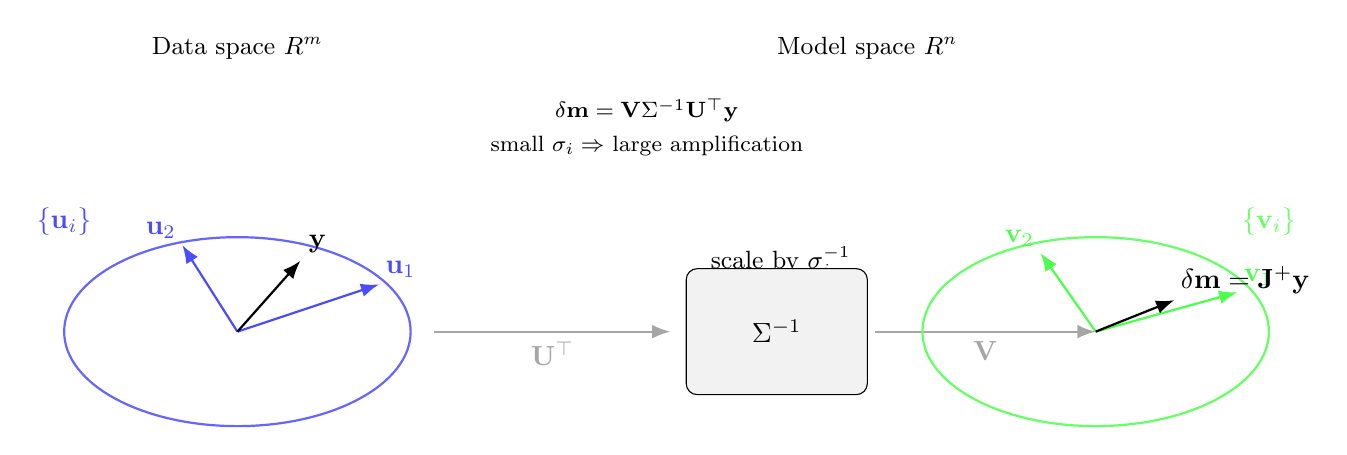
\begin{tikzpicture}[scale=1.0,>=Latex]
  % Labels
  \node at (0,3.6) {\small Data space $\mathbb{R}^m$};
  \node at (8,3.6) {\small Model space $\mathbb{R}^n$};

  % Ellipse in data space showing left singular vectors
  \draw[thick,blue!60] (0,0) ellipse (2.2cm and 1.2cm);
  \node[blue!70] at (-2.2,1.4) {$\{\mathbf{u}_i\}$};

  % Basis vectors u1, u2 drawn
  \draw[->,thick,blue!70] (0,0) -- (1.8,0.6) node[above right=-2pt] {$\mathbf{u}_1$};
  \draw[->,thick,blue!70] (0,0) -- (-0.7,1.1) node[above left=-2pt] {$\mathbf{u}_2$};

  % Data vector y
  \coordinate (Y) at (0.8,0.9);
  \draw[->,thick] (0,0) -- (Y) node[above right=-1pt] {$\mathbf{y}$};

  % Arrow showing mapping by U^T
  \draw[->,gray!70,thick] (2.5,0.0) -- (5.5,0.0) node[midway,below] {$\mathbf{U}^\top$};

  % Middle panel: singular value scaling
  \node at (6.9,0.9) {\small scale by $\sigma_i^{-1}$};
  \draw[fill=gray!10,rounded corners] (5.7,-0.8) rectangle (8.0,0.8);
  \node at (6.85,0.0) {$\bm{\Sigma}^{-1}$};

  % Arrow to model space
  \draw[->,gray!70,thick] (8.1,0.0) -- (10.9,0.0) node[midway,below] {$\mathbf{V}$};

  % Model space ellipse showing right singular vectors v_i
  \begin{scope}[shift={(8,0)}]
    \draw[thick,green!60] (2.9,0) ellipse (2.2cm and 1.2cm);
    \node[green!60] at (5.1,1.4) {$\{\mathbf{v}_i\}$};
    \draw[->,thick,green!70] (2.9,0) -- (4.7,0.5) node[above right=-2pt] {$\mathbf{v}_1$};
    \draw[->,thick,green!70] (2.9,0) -- (2.2,1.0) node[above left=-2pt] {$\mathbf{v}_2$};
    % Solution vector delta m
    \coordinate (M) at (3.9,0.4);
    \draw[->,thick] (2.9,0) -- (M) node[above right=-2pt] {$\delta\mathbf{m}=\mathbf{J}^+\mathbf{y}$};
  \end{scope}

  % Notes
  \node[align=center] at (5.2,2.6) {\footnotesize $\delta\mathbf{m}=\mathbf{V}\bm{\Sigma}^{-1}\mathbf{U}^\top\mathbf{y}$\\
  \footnotesize small $\sigma_i \Rightarrow$ large amplification};
\end{tikzpicture}
\caption{Pseudoinverse via SVD: project $\mathbf{y}$ onto $\{\mathbf{u}_i\}$, scale by $1/\sigma_i$, then map into model space via $\{\mathbf{v}_i\}$.}
\end{figure}

\subsection{Regularization}\label{subsec:reg}
When $\mathbf{J}$ is ill-conditioned or rank-deficient, we stabilize the inversion by augmenting the objective with prior information or penalties.

\subsubsection{Tikhonov ($\ell_2$) Regularization}
\paragraph{Zero-order (ridge).}
\[
\min_{\delta\mathbf{m}} \; \|\mathbf{y}-\mathbf{J}\delta\mathbf{m}\|_2^2 + \lambda^2 \,\|\delta\mathbf{m}\|_2^2.
\]
Normal equations:
\[
\left(\mathbf{J}^\top \mathbf{J} + \lambda^2 \mathbf{I}\right)\delta\mathbf{m} = \mathbf{J}^\top \mathbf{y}.
\]
SVD filter factors:
\[
\delta\mathbf{m}_\lambda = \sum_{i=1}^r \frac{\sigma_i}{\sigma_i^2+\lambda^2}\,(\mathbf{u}_i^\top \mathbf{y})\,\mathbf{v}_i,\qquad
\phi_i(\lambda)=\frac{\sigma_i}{\sigma_i^2+\lambda^2}.
\]
Small singular directions are damped smoothly as $\sigma_i \downarrow 0$.

\paragraph{General-order (with roughness operator).}
Let $\mathbf{L}$ encode roughness (e.g., discrete gradient or Laplacian on the model):
\[
\min_{\delta\mathbf{m}} \; \|\mathbf{y}-\mathbf{J}\delta\mathbf{m}\|_2^2 + \lambda^2 \,\|\mathbf{L}\,\delta\mathbf{m}\|_2^2,
\]
with normal equations $\big(\mathbf{J}^\top \mathbf{J} + \lambda^2 \mathbf{L}^\top \mathbf{L}\big)\,\delta\mathbf{m} = \mathbf{J}^\top \mathbf{y}$. This biases solutions toward smoothness or other desired structure.

\subsubsection{Levenberg--Marquardt (Damped Gauss--Newton)}
For nonlinear problems, LM solves
\[
\left(\mathbf{J}^\top\mathbf{J} + \lambda^2 \mathbf{D}\right)\delta\mathbf{m} = \mathbf{J}^\top \mathbf{r},
\]
with $\mathbf{D}$ often chosen as $\mathrm{diag}(\mathbf{J}^\top \mathbf{J})$ (Marquardt) or $\mathbf{I}$ (Levenberg). The damping $\lambda$ is adapted: large $\lambda$ gives gradient-descent-like steps; small $\lambda$ recovers Gauss--Newton near the solution.

\subsection{Weighted Least Squares (WLS) and Generalized Pseudoinverse}\label{subsec:wls}
Assume data covariance $\mathbf{C}_d \succ 0$. The WLS objective is
\[
\min_{\delta\mathbf{m}}\; \|\mathbf{y}-\mathbf{J}\,\delta\mathbf{m}\|_{\mathbf{C}_d^{-1}}^2 := (\mathbf{y}-\mathbf{J}\,\delta\mathbf{m})^\top \mathbf{C}_d^{-1} (\mathbf{y}-\mathbf{J}\,\delta\mathbf{m}).
\]
\paragraph{Whitening.} Let $\mathbf{W}$ satisfy $\mathbf{W}^\top\mathbf{W}=\mathbf{C}_d^{-1}$ (e.g., $\mathbf{W}=\mathbf{C}_d^{-1/2}$). Define $\tilde{\mathbf{y}}=\mathbf{W}\mathbf{y}$ and $\tilde{\mathbf{J}}=\mathbf{W}\mathbf{J}$. Then
\[
\min_{\delta\mathbf{m}} \; \|\tilde{\mathbf{y}}-\tilde{\mathbf{J}}\,\delta\mathbf{m}\|_2^2,
\]
with normal equations $\tilde{\mathbf{J}}^\top\tilde{\mathbf{J}}\,\delta\mathbf{m}=\tilde{\mathbf{J}}^\top \tilde{\mathbf{y}}$, i.e.,
\[
(\mathbf{J}^\top \mathbf{C}_d^{-1} \mathbf{J})\,\delta\mathbf{m} = \mathbf{J}^\top \mathbf{C}_d^{-1} \mathbf{y}.
\]
The minimum-norm WLS solution is
\[
\delta\mathbf{m}_\ast = (\mathbf{J}^\top \mathbf{C}_d^{-1} \mathbf{J})^{+} \mathbf{J}^\top \mathbf{C}_d^{-1} \mathbf{y} \,=\, (\tilde{\mathbf{J}})^{+}\,\tilde{\mathbf{y}}.
\]
\paragraph{Weighted projector.} The fitted data are $\widehat{\mathbf{y}}=\mathbf{J}\,\delta\mathbf{m}_\ast$, and the $\mathbf{C}_d^{-1}$-orthogonal projector onto $\mathcal{R}(\mathbf{J})$ is
\[
\mathbf{P}_{\mathcal{R}(\mathbf{J});\,\mathbf{C}_d^{-1}} = \mathbf{J} (\mathbf{J}^\top \mathbf{C}_d^{-1} \mathbf{J})^{+} \mathbf{J}^\top \mathbf{C}_d^{-1},
\]
which is idempotent and self-adjoint in the $\langle\cdot,\cdot\rangle_{\mathbf{C}_d^{-1}}$ inner product.

\paragraph{Minimum-\(\mathbf{C}_m^{-1}\)-norm WLS solution.} If one prefers the solution of minimal $\|\delta\mathbf{m}\|_{\mathbf{C}_m^{-1}} := (\delta\mathbf{m})^\top \mathbf{C}_m^{-1} (\delta\mathbf{m})$ among all WLS minimizers (with $\mathbf{C}_m\succ 0$), then under whitening the solution is
\[
\delta\mathbf{m}_\ast = \mathbf{C}_m \tilde{\mathbf{J}}^\top\,\big(\tilde{\mathbf{J}}\,\mathbf{C}_m\,\tilde{\mathbf{J}}^\top\big)^{+}\,\tilde{\mathbf{y}} \,=\, \mathbf{C}_m \mathbf{J}^\top \mathbf{W}^\top\,\big(\mathbf{W}\mathbf{J}\,\mathbf{C}_m\,\mathbf{J}^\top\mathbf{W}^\top\big)^{+}\,\mathbf{W}\mathbf{y}.
\]
This is the generalized (metric-weighted) pseudoinverse mapping from data to parameters under the data inner product induced by $\mathbf{C}_d^{-1}$ and the model inner product induced by $\mathbf{C}_m^{-1}$.

\subsection{Gauss--Newton vs. Levenberg--Marquardt: Trust-Region View}
Let $\mathbf{g}=\mathbf{J}^\top\mathbf{r}$ and $\mathbf{H}=\mathbf{J}^\top\mathbf{J}$. Gauss--Newton uses $\mathbf{H}\,\delta\mathbf{m}_{\text{GN}}=\mathbf{g}$, while LM uses $(\mathbf{H}+\lambda^2\mathbf{D})\,\delta\mathbf{m}_{\text{LM}}=\mathbf{g}$ with $\lambda\ge 0$ and positive definite $\mathbf{D}$.

\begin{figure}[h!]
\centering
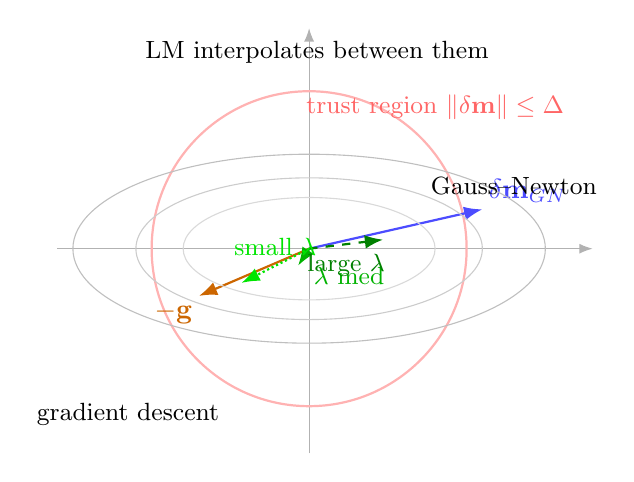
\begin{tikzpicture}[scale=1.0,>=Latex]
  % Axes in model space
  \draw[->,gray!60] (-3.2,0) -- (3.6,0);
  \draw[->,gray!60] (0,-2.6) -- (0,2.8);

  % Trust-region circle
  \draw[red!30,thick] (0,0) circle [radius=2.0];
  \node[red!60] at (1.6,1.8) {\small trust region $\|\delta\mathbf{m}\|\le \Delta$};

  % Define origin and key directions
  \coordinate (O) at (0,0);
  \coordinate (g) at (-1.4,-0.6); % -g is descent
  \coordinate (sgn) at (2.2,0.5);  % GN step example

  % Gradient descent direction (-g)
  \draw[->,thick,orange!80!black] (O) -- (g) node[below left=-2pt] {$-\mathbf{g}$};

  % GN step
  \draw[->,thick,blue!70] (O) -- (sgn) node[above right=-2pt] {$\delta\mathbf{m}_{\text{GN}}$};

  % LM steps for different lambdas: interpolate between sgn and g
  \draw[->,thick,green!70!black]          (O) -- ($(sgn)!0.65!(g)$) node[midway,below right] {\small $\lambda$ med};
  \draw[->,thick,green!50!black,dashed]   (O) -- ($(sgn)!0.35!(g)$) node[midway,below]       {\small large $\lambda$};
  \draw[->,thick,green!90!black,densely dotted] (O) -- ($(sgn)!0.85!(g)$) node[midway,above] {\small small $\lambda$};

  % Elliptic contours of quadratic model
  \draw[gray!50] (0,0) ellipse (3.0cm and 1.2cm);
  \draw[gray!40] (0,0) ellipse (2.2cm and 0.9cm);
  \draw[gray!30] (0,0) ellipse (1.6cm and 0.65cm);

  % Labels
  \node at (-2.3,-2.1) {\small gradient descent};
  \node at (2.6,0.8)   {\small Gauss--Newton};
  \node at (0.1,2.5)   {\small LM interpolates between them};
  \end{tikzpicture}
  \caption{LM step interpolates between gradient descent ($\lambda\to\infty$) and Gauss--Newton ($\lambda\to 0$). Trust-region interpretations adapt $\lambda$ to keep steps within a radius $\Delta$.}
\end{figure}

\subsection{TikZ: Normal vs. Regularized Normal Equations}
\begin{figure}[h!]
\centering
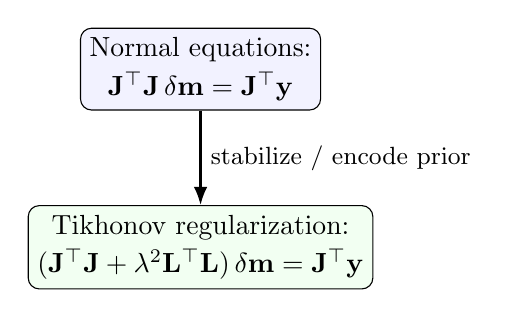
\begin{tikzpicture}[>=Latex]
  \node[draw,rounded corners,fill=blue!5,align=center] (NE)
    {Normal equations:\\[2pt]
     $\mathbf{J}^\top\mathbf{J}\,\delta\mathbf{m}=\mathbf{J}^\top\mathbf{y}$};

  \node[draw,rounded corners,fill=green!5,align=center,below=1.2cm of NE] (REG)
    {Tikhonov regularization:\\[2pt]
     $(\mathbf{J}^\top\mathbf{J}+\lambda^2\mathbf{L}^\top\mathbf{L})\,\delta\mathbf{m}=\mathbf{J}^\top\mathbf{y}$};

  \draw[->,thick] (NE) -- (REG) node[midway,right] {\small stabilize / encode prior};
\end{tikzpicture}
\caption{Regularization augments the normal equations to improve conditioning and encode prior structure.}
\end{figure}

\subsection{Choosing \texorpdfstring{$\lambda$}{lambda}}
Common strategies: (i) \emph{L-curve}: plot $\log \|\mathbf{y}-\mathbf{J}\delta\mathbf{m}_\lambda\|$ vs. $\log \|\mathbf{L}\delta\mathbf{m}_\lambda\|$ and pick the corner; (ii) \emph{Generalized Cross-Validation (GCV)}: minimize a predictive risk proxy (especially for $\ell_2$); (iii) \emph{Discrepancy Principle}: choose $\lambda$ so the residual norm matches the expected noise level.

\subsection{Intermediate Derivations (Expanded)}
\paragraph{Gradient and Hessian of the linearized objective.}
\[
\Phi(\delta\mathbf{m}) = \|\mathbf{y}-\mathbf{J}\delta\mathbf{m}\|_2^2
= (\mathbf{y}-\mathbf{J}\delta\mathbf{m})^\top(\mathbf{y}-\mathbf{J}\delta\mathbf{m}).
\]
Then $\nabla \Phi = -2\,\mathbf{J}^\top (\mathbf{y}-\mathbf{J}\delta\mathbf{m}) = -2\,\mathbf{J}^\top \mathbf{y} + 2\,\mathbf{J}^\top\mathbf{J}\,\delta\mathbf{m}$ and $\nabla^2 \Phi = 2\,\mathbf{J}^\top \mathbf{J}$. Setting $\nabla\Phi=\mathbf{0}$ recovers the normal equations.

\paragraph{WLS normal equations via whitening.} With $\mathbf{W}^\top\mathbf{W}=\mathbf{C}_d^{-1}$, minimizing $\|\mathbf{W}(\mathbf{y}-\mathbf{J}\delta\mathbf{m})\|_2^2$ yields $\tilde{\mathbf{J}}^\top\tilde{\mathbf{J}}\,\delta\mathbf{m}=\tilde{\mathbf{J}}^\top \tilde{\mathbf{y}}$, equivalent to $\mathbf{J}^\top \mathbf{C}_d^{-1} \mathbf{J}\,\delta\mathbf{m}=\mathbf{J}^\top \mathbf{C}_d^{-1} \mathbf{y}$.

\paragraph{Projection operator relations.} The orthogonal projector (Euclidean) is $\mathbf{P}=\mathbf{J}\mathbf{J}^+$. In WLS, the $\mathbf{C}_d^{-1}$-orthogonal projector is $\mathbf{P}_{\mathbf{C}_d^{-1}}=\mathbf{J} (\mathbf{J}^\top \mathbf{C}_d^{-1} \mathbf{J})^{+} \mathbf{J}^\top \mathbf{C}_d^{-1}$, which is idempotent and self-adjoint in the weighted inner product.

\paragraph{Bayesian/Tikhonov equivalence.} With Gaussian priors $\delta\mathbf{m}\sim\mathcal{N}(\mathbf{0},\mathbf{C}_m)$ and data noise $\mathcal{N}(\mathbf{0},\mathbf{C}_d)$, the MAP estimate solves $(\mathbf{J}^\top \mathbf{C}_d^{-1}\mathbf{J}+\mathbf{C}_m^{-1})\,\delta\mathbf{m}=\mathbf{J}^\top \mathbf{C}_d^{-1}\mathbf{y}$; posterior covariance is $(\mathbf{J}^\top \mathbf{C}_d^{-1}\mathbf{J}+\mathbf{C}_m^{-1})^{-1}$.

\subsection{Practical Notes}
\begin{itemize}
  \item \textbf{Scaling}: Normalize columns of $\mathbf{J}$ and/or parameters to balance sensitivities.
  \item \textbf{Whitening}: Prewhiten with $\mathbf{C}_d^{-1/2}$ so residuals are in standard deviation units.
  \item \textbf{Rank-revealing factorizations}: Use SVD or QR with column pivoting to detect rank deficiency and guide TSVD or damping.
  \item \textbf{Stopping}: relative step size $\|\delta\mathbf{m}\|/\|\mathbf{m}\|$, relative residual decrease, and/or gradient norm $\|\mathbf{J}^\top \mathbf{r}\|$.
\end{itemize}

\subsection*{References}
\begin{itemize}
  \item G. H. Golub and C. F. Van Loan, \emph{Matrix Computations}, 4th ed., JHU Press, 2013 (SVD, pseudoinverse, conditioning).
  \item Å. Björck, \emph{Numerical Methods for Least Squares Problems}, SIAM, 1996 (LS, WLS, regularization, algorithms).
  \item R. A. Horn and C. R. Johnson, \emph{Matrix Analysis}, 2nd ed., Cambridge Univ. Press, 2012 (projections, generalized inverses).
  \item R. C. Aster, B. Borchers, and C. H. Thurber, \emph{Parameter Estimation and Inverse Problems}, 3rd ed., Elsevier, 2019 (inverse problems, Tikhonov, LM, Bayesian view).
\end{itemize}


\end{document}
